CDMS lead: Francisco Ponce
\begin{figure}
\begin{center}
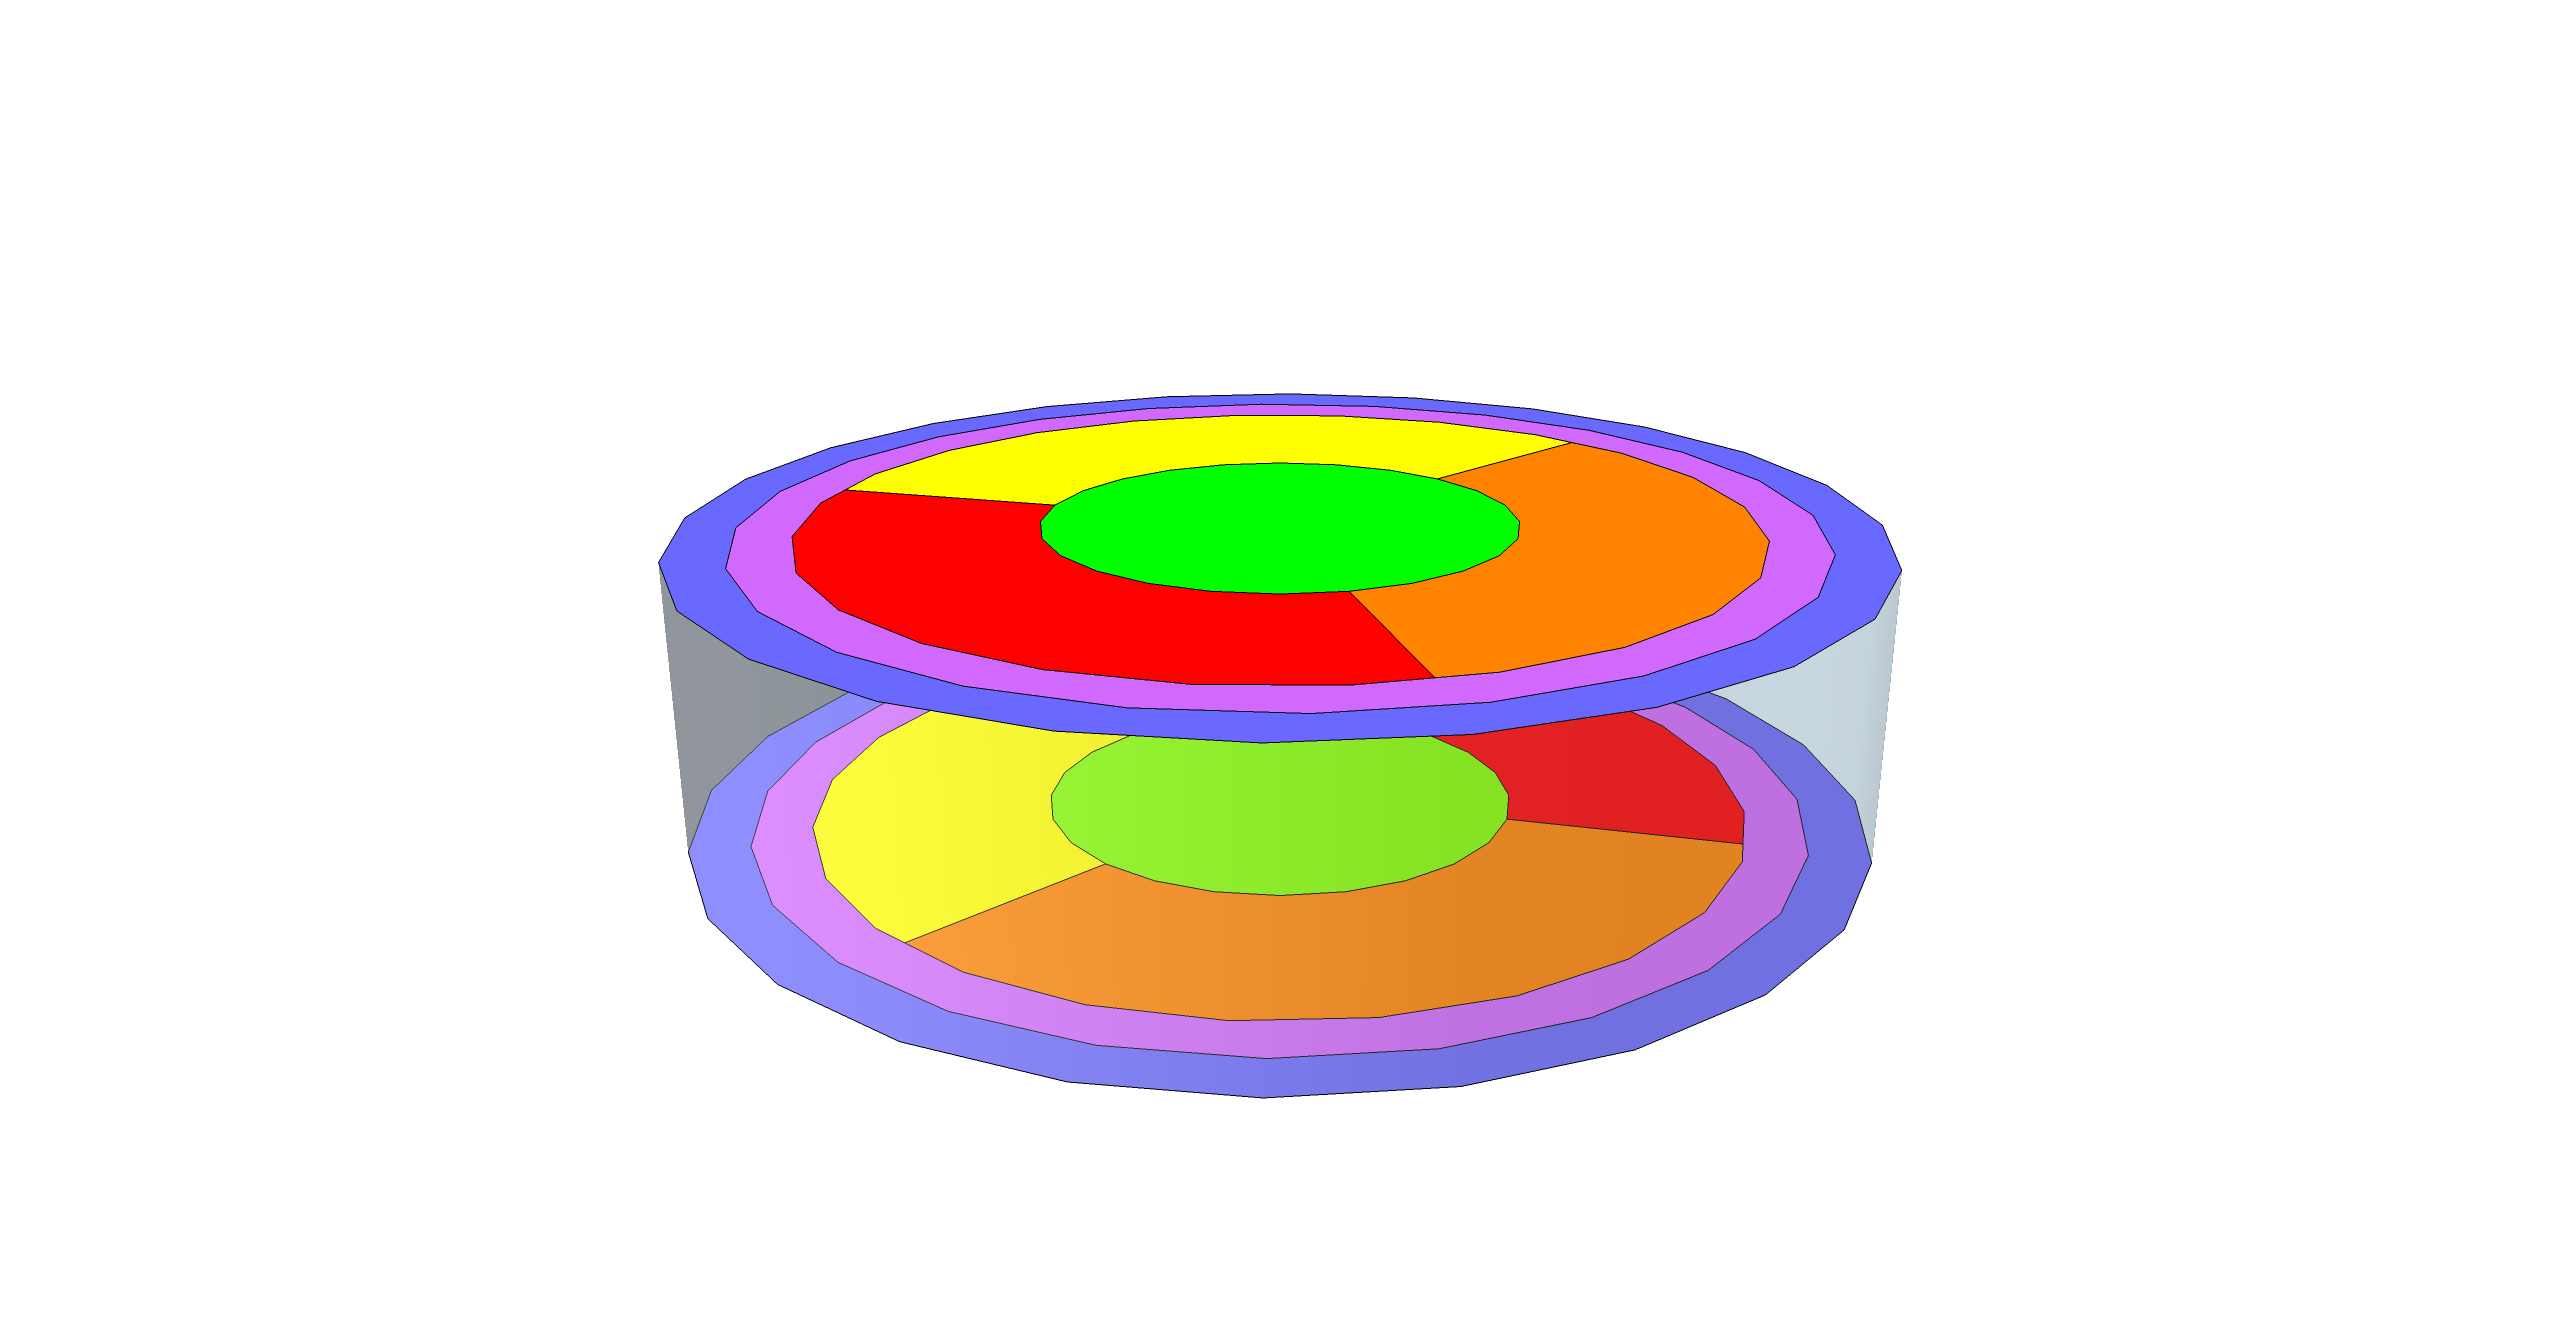
\includegraphics[width=.45\textwidth, trim={600 200 600 350},clip]{figures/f01a_HV_Detector_Schematic.png}
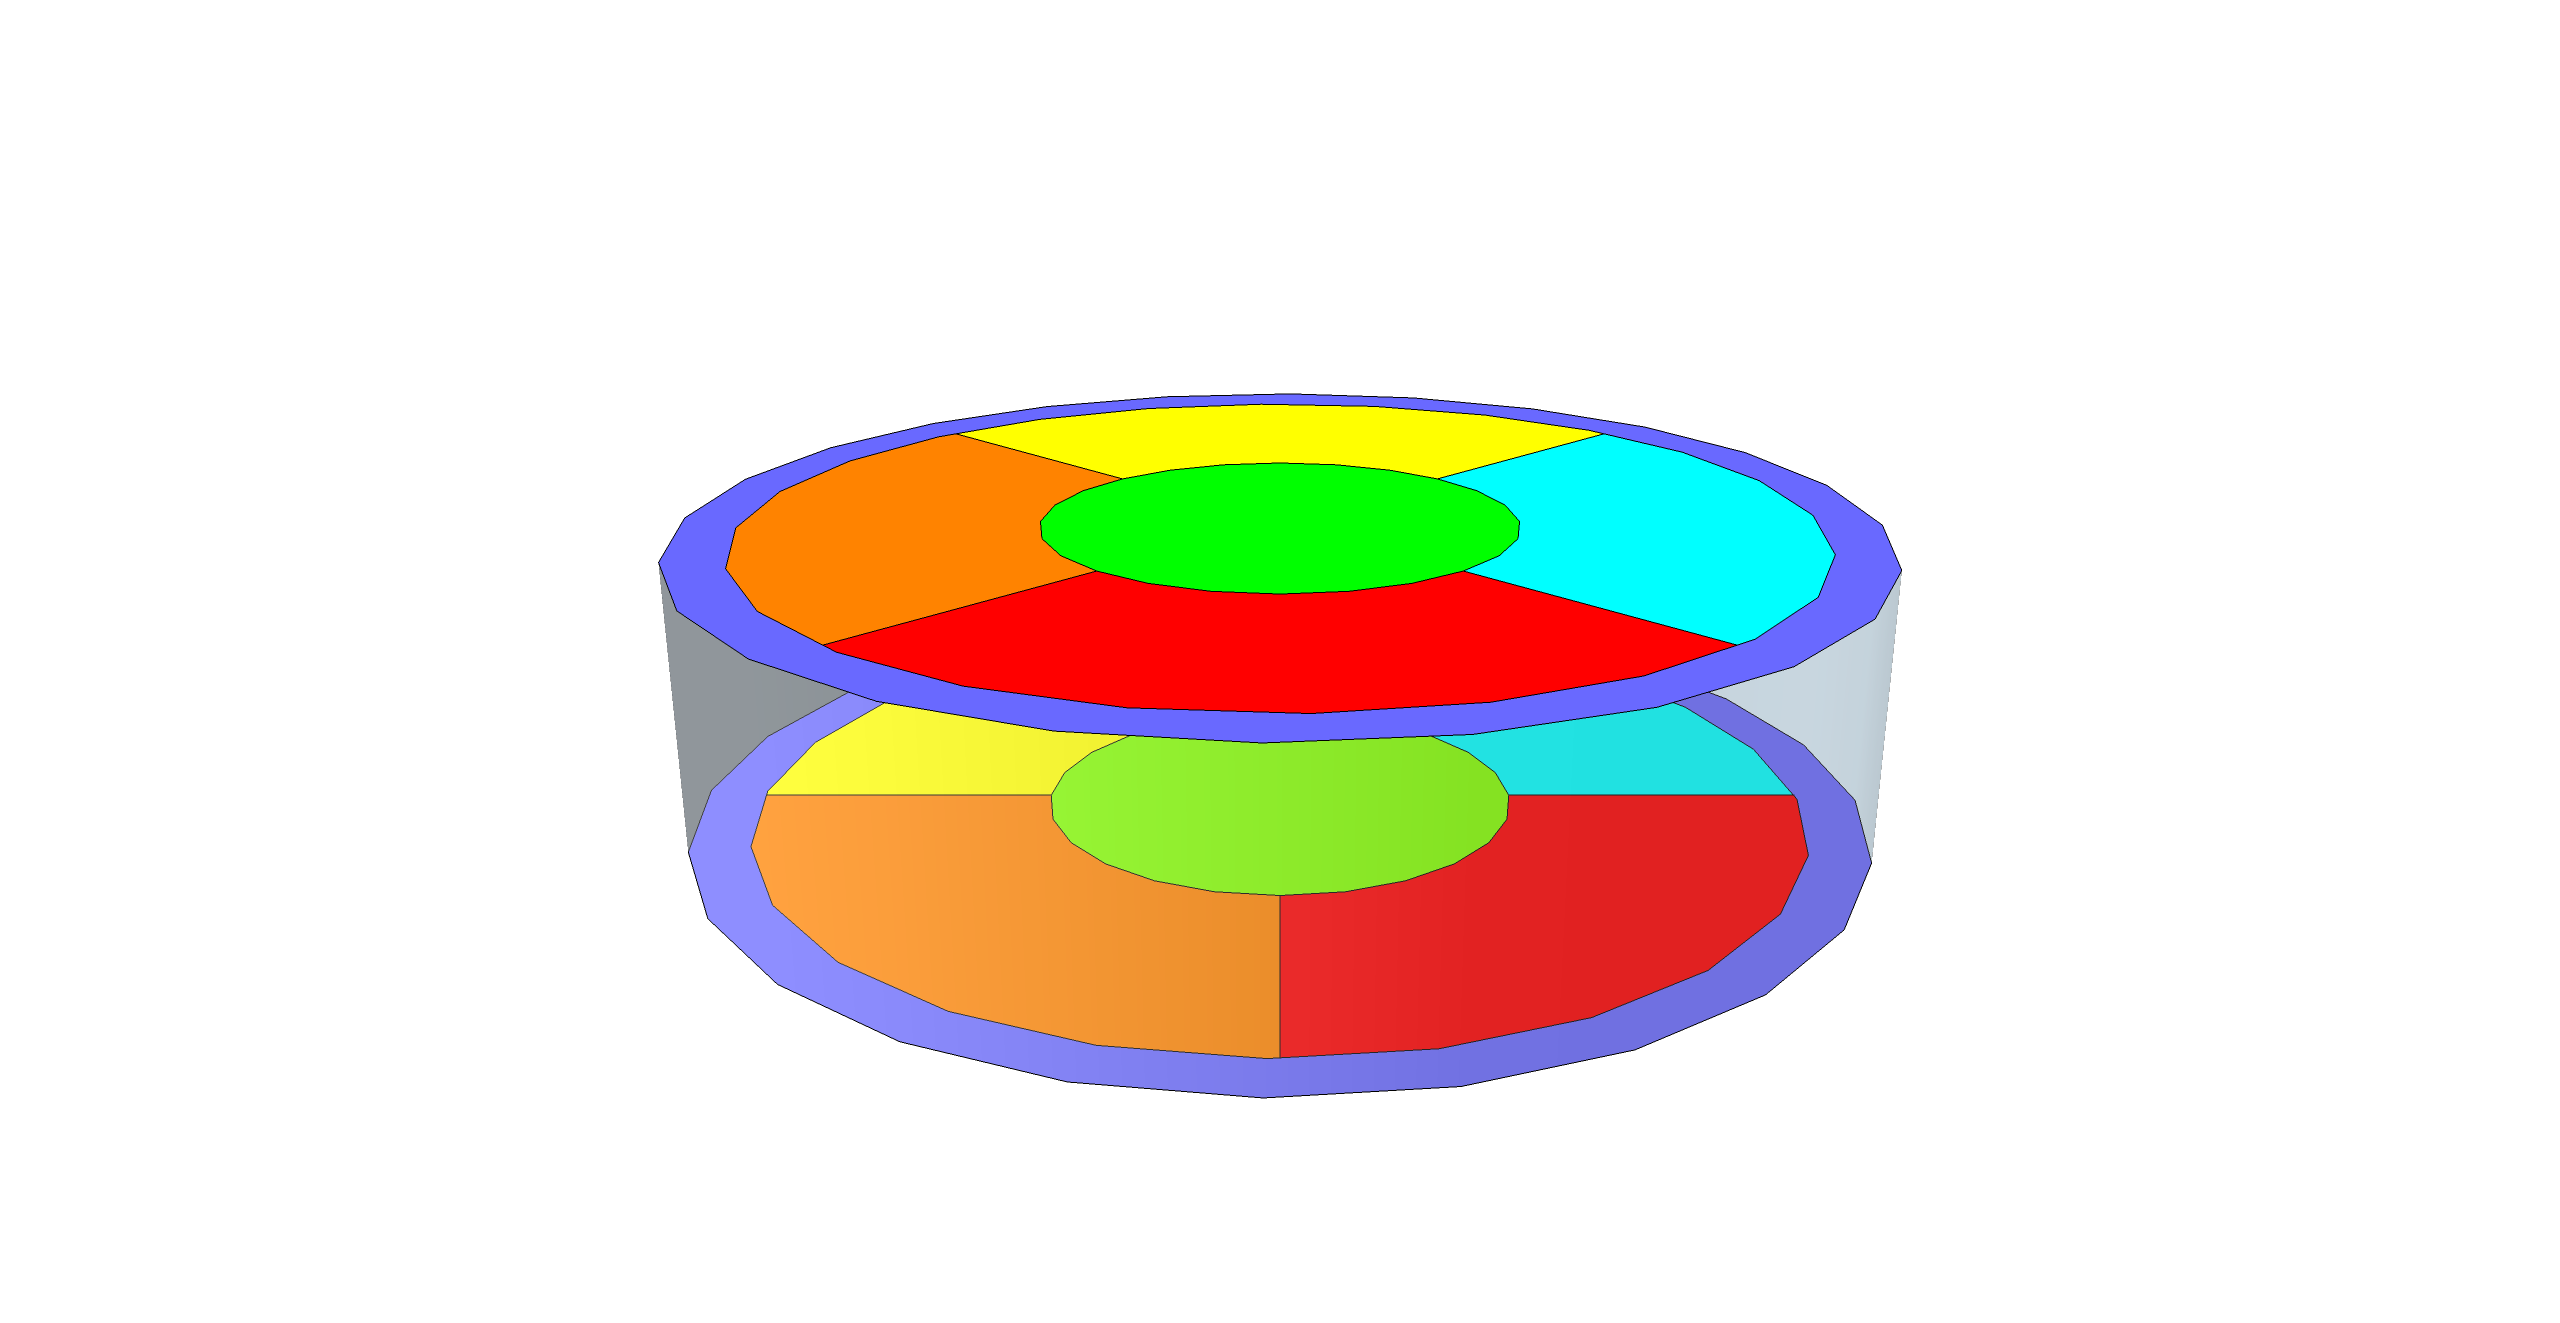
\includegraphics[width=.45\textwidth, trim={600 200 600 350},clip]{figures/f01b_iZIP_Detector_Schematic.png}
\end{center}
\caption{Channel layout for the HV (left) and iZIP (right) detectors. The HV detector has six phonon channels on each side: an inner ``core'' surrounded by three wedge-shaped channels and two outer rings designed to reject events near the edge. Each channel contains hundreds of lithographically defined superconducting sensors. The wedge channels on the bottom surface are rotated by 60$^\circ$ with respect to those on the top.
The interleaved Z-sensitive Ionization Phonon (iZIP) detector also has six phonon channels on each side, arranged as an inner core surrounded by four wedge shaped channels and one outer ring. An ``outer'' ionization channel shares the same area and is interleaved with the outermost phonon ring, and an ``inner'' ionization channel is interleaved with the remaining phonon channels. The wedge channels on the bottom surface are rotated by 45$^\circ$ with respect to those on the top. \it{Reproduced from ~\cite{SCDMS2017}}}
\label{fig:SCDMS_Detectors}
\end{figure}

The Super Cryogenic Dark Matter Search (SuperCDMS) SNOLAB experiment is a 2$^{nd}$ generation dark matter experiment, which will commission its solid-state detectors 2 km underground at the SNOLAB facility in Sudbury, Canada. The solid-state detectors are 100 mm diameter, 33.3 mm thick germanium or silicon crystals patterned with both Quasiparticle-assisted Electrothermal-feedback Transition edge sensors (QETs) as phonon sensors and electrodes used for charge readout and/or biasing the crystal on both 100 mm faces. The patterned QETs and electrodes are optimized to operate as either High Voltage (HV) or interleaved Z-dependent Ionization and Phonon (iZIP) detector, see Figure ~\ref{fig:SCDMS_Detectors}. 
As a HV detector, the electrodes are used to apply a relatively large bias voltage, V$_b$, across the crystal. The applied voltage gives rise to an \textbf{E}-field that causes electrons and holes to drift to opposing faces of the detector. While drifting the charges scatter off the crystal lattice generating additional phonons via the Neganov-Trofimov-Luke (NTL) effect ~\cite{Neganov1985, Luke1988}. The resulting total energy observed by the QETs on the detector faces is
\begin{equation}
    E_{tot} = E_r + N_{eh}eV_{b}
\end{equation}
Where E$_r$ is the initial recoil energy, and N$_{eh}$ is the number of electron-hole pairs initially created. These devices have an improved ultra-high resolution and reach lower thresholds allowing them to probe lower DM masses. Unfortunately, this improvement comes with a loss in electron recoil (ER) to nuclear recoil (NR) discrimination, and surface event rejection. Nonetheless, the HV detectors are expected to explore WIMP DM masses down to ~0.3 GeV. 
As an iZIP detector, the electrodes are used as charge collectors as well as to bias the crystal at lower voltages compared to the HV detector. These detectors measure both prompt phonons and ionization charge signals, which can be used to perform ER/NR discrimination based on the difference in ionization yield. Furthermore, optimization of the electrode layout allow identification of surface events via a charge signal collection asymmetry: bulk (nominally symmetric signals) and surface (heavily asymmetric signals) events. This allows rejection of beta particle and further reduces the background in the operation of these devices. The advanced rejection capabilities of these devices project sensitivities in a “background-free” mode to WIMPs with masses $>$5 GeV and in a “limited-discrimination” mode to WIMPS $>$1 GeV~\cite{SCDMS2017}.

The SuperCDMS SNOLAB experiment anticipates observing approximately 50 events associated with neutrino interactions but will not reach the neutrino fog [\textbf{ref, add plots here}]. To get the sensitivity required to reach the neutrino fog both backgrounds and detector improvements are needed. In terms of backgrounds the improvements already under R\&D appear to be sufficient in reaching the neutrino fog given a certain level of detector improvements. The background improvements include sourcing new material and replacing components with lower background alternatives, and improving detector fabrication/tower assembly to reduce the $^{210}$Pb plated onto the surface from radon. The R\&D for these changes is mature and thus the cost to implement is expected to be low. 

Proposed detector upgrades common to both HV and iZIP style detectors include 1) smaller detector sizes, 2) lowering the TES critical temperature (T$_C$), and 3) improving phonon transmission across interfaces. 

Scaling to smaller detectors will improve the phonon/ionization resolution of the SuperCDMS detectors, which in turn will improve rejection of bulk ER backgrounds. This development is reasonably mature with prototype Si HVeV detectors (an HV style device) already deployed at test facilities ~\cite{SCDMS2019,SCDMS2020}. R\&D efforts are set to shift toward the development of a Ge HVeV detector and optimization of these devices. As such a change in detector size to 10 cm$^3$ (3x3x1.2 cm$^3$) or 1 cm$^3$ (1x1x0.4 cm$^3$) is readily achievable. In addition, to the cost to finalize this R\&D there is also a one-time cost to redesign the detector tower to accommodate several of the new size detectors in the same volume and the corresponding readout cables.

Lowering of the TES T$_C$ is less mature, but a viable path forward is known. The thin tungsten film that is at the heart of the QET can grow in two different phases, $\alpha$-W with a T$_C$ of 15 mK or $\beta$-W with a T$_C$ over 2 K, during deposition. By mixing these two phases in different ratios the T$_C$ can be tuned between the two extremes. The challenge is in identifying the proper deposition parameters under which the W film will grow at the proper ratio in a reproducible and controllable manner. This will require some financial investment to characterize a deposition system, which include man hours to test the resulting films. As a first level improvement a T$_C$ of 40 mK is considered reasonably achievable. This change will incur one-time cost of fabricating new detectors (in addition to any cost from a change to the detector size).

Improvements in phonon transmission from the crystal all the way to the W TES is the least mature advancement being considered, with no immediate avenues forward identified. 

